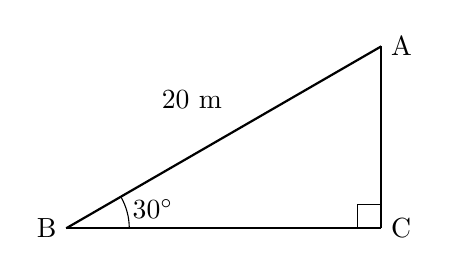
\begin{tikzpicture}

% Define coordinates for the right triangle
\coordinate (B) at (0,0);          % Bottom left vertex
\coordinate (C) at (4,0);          % Bottom right vertex (right angle)
\coordinate (A) at (4,2.31);       % Top right vertex (maintaining 30° at B)

% Draw the triangle sides
\draw[thick] (B) -- (A);           % Hypotenuse BA
\draw[thick] (A) -- (C);           % Vertical side AC
\draw[thick] (C) -- (B);           % Horizontal side CB

% Draw the right angle symbol at C
\draw (3.7,0) -- (3.7,0.3) -- (4,0.3);

% Draw the arc for 30° angle at B
\draw (0.8,0) arc[start angle=0, end angle=30, radius=0.8];

% Label the 30° angle
\node at (1.1,0.25) {$30^{\circ}$};

\node[above left] at (2.1,1.4) {$20$ m};

% Label all vertices
\node[left] at (B) {B};
\node[right] at (C) {C};
\node[right] at (A) {A};

\end{tikzpicture}